The average RF rates of different variants of ASTRAL and wQFM on various model conditions in 15-taxon dataset are shown in Fig.~\ref{fig:RF_Rates_15_taxon}. We have investigated the performance on varying gene tree estimation errors using 100bp and 1000bp sequence lengths and on varying numbers of genes (100 and 1000). In general, wQFM is more accurate than ASTRAL both on complete and incomplete gene trees. For all levels of missing data, certain trends were clearly seen. As expected, tree accuracy of ASTRAL and wQFM deteriorated in the presence of missing taxa, and the RF rates increased with increasing levels of missing data. However, tree accuracy of ASTRAL is more impacted by increasing levels of missing data than that of wQFM as wQFM-incomplete was notably better than ASTRAL-incomplete on most of the model conditions (especially, see the results on 100gene-1000bp and 1000gene-100bp model conditions) and in many cases, the differences are statistically significant ($p \ll 0.05$). ASTRAL and wQFM improves in accuracy as the number of genes increased (from 100 to 1000) and often achieved competitive tree accuracy (compared to the accuracy of the trees estimated on complete gene trees) even when the amount of missing data was large. This is mostly due to the fact that a  large number of gene trees provide more unique bipartitions (and hence more quartets) than a relatively smaller number of genes.


The most important and interesting results were observed on imputed sets of quartets. wQFM-imputed substantially outperformed not only wQFM-incomplete and ASTRAL-incomplete but also wQFM-complete and ASTRAL-complete, showing the efficacy of QT-GILD in imputing quartet distributions. The improvements are remarkable as in most of the model conditions, wQFM-imputed returned the true species tree (RF-rate = 0), whereas ASTRAL-incomplete and wQFM-incomplete incurred as high as $\sim$45\% errors (note the higher taxa removal rates on 100gene-100bp model condition). Note that, even with a reasonably well imputed set of quartets, the expected trend is for the accuracy of the tree estimated on an imputed set of quartets to be higher than that of the tree estimated on the corresponding incomplete quartet distribution but lower than or as good as the tree accuracy obtained on the complete quartet distribution. But, surprisingly, wQFM-imputed improves upon wQFM-complete (as well as ASTRAL-complete) on this particular dataset. These results suggest, and as we will show in the following, that the imputed quartet distributions are closer to true quartet distributions than the complete and incomplete quartet distributions are to true distributions. Note that, on the 100gene-100bp model condition, the RF rates of the trees estimated on imputed quartets with 1-2 missing taxa were higher than those with larger amounts of missing data. 
We believe this is because there are only 18272.8 missing quartets with 1-2 missing taxa, and thus QT-GILD could not account for gene tree estimation error as much as it did in other model conditions with larger numbers of missing quartets.
% \addb{not sure what can we say here as an explanation. This is not clear why but we think that the self-supervisions module with feedback loop did not have enough missing entry to impute ..}



\begin{figure}[htpb]
    \centering % <-- added
    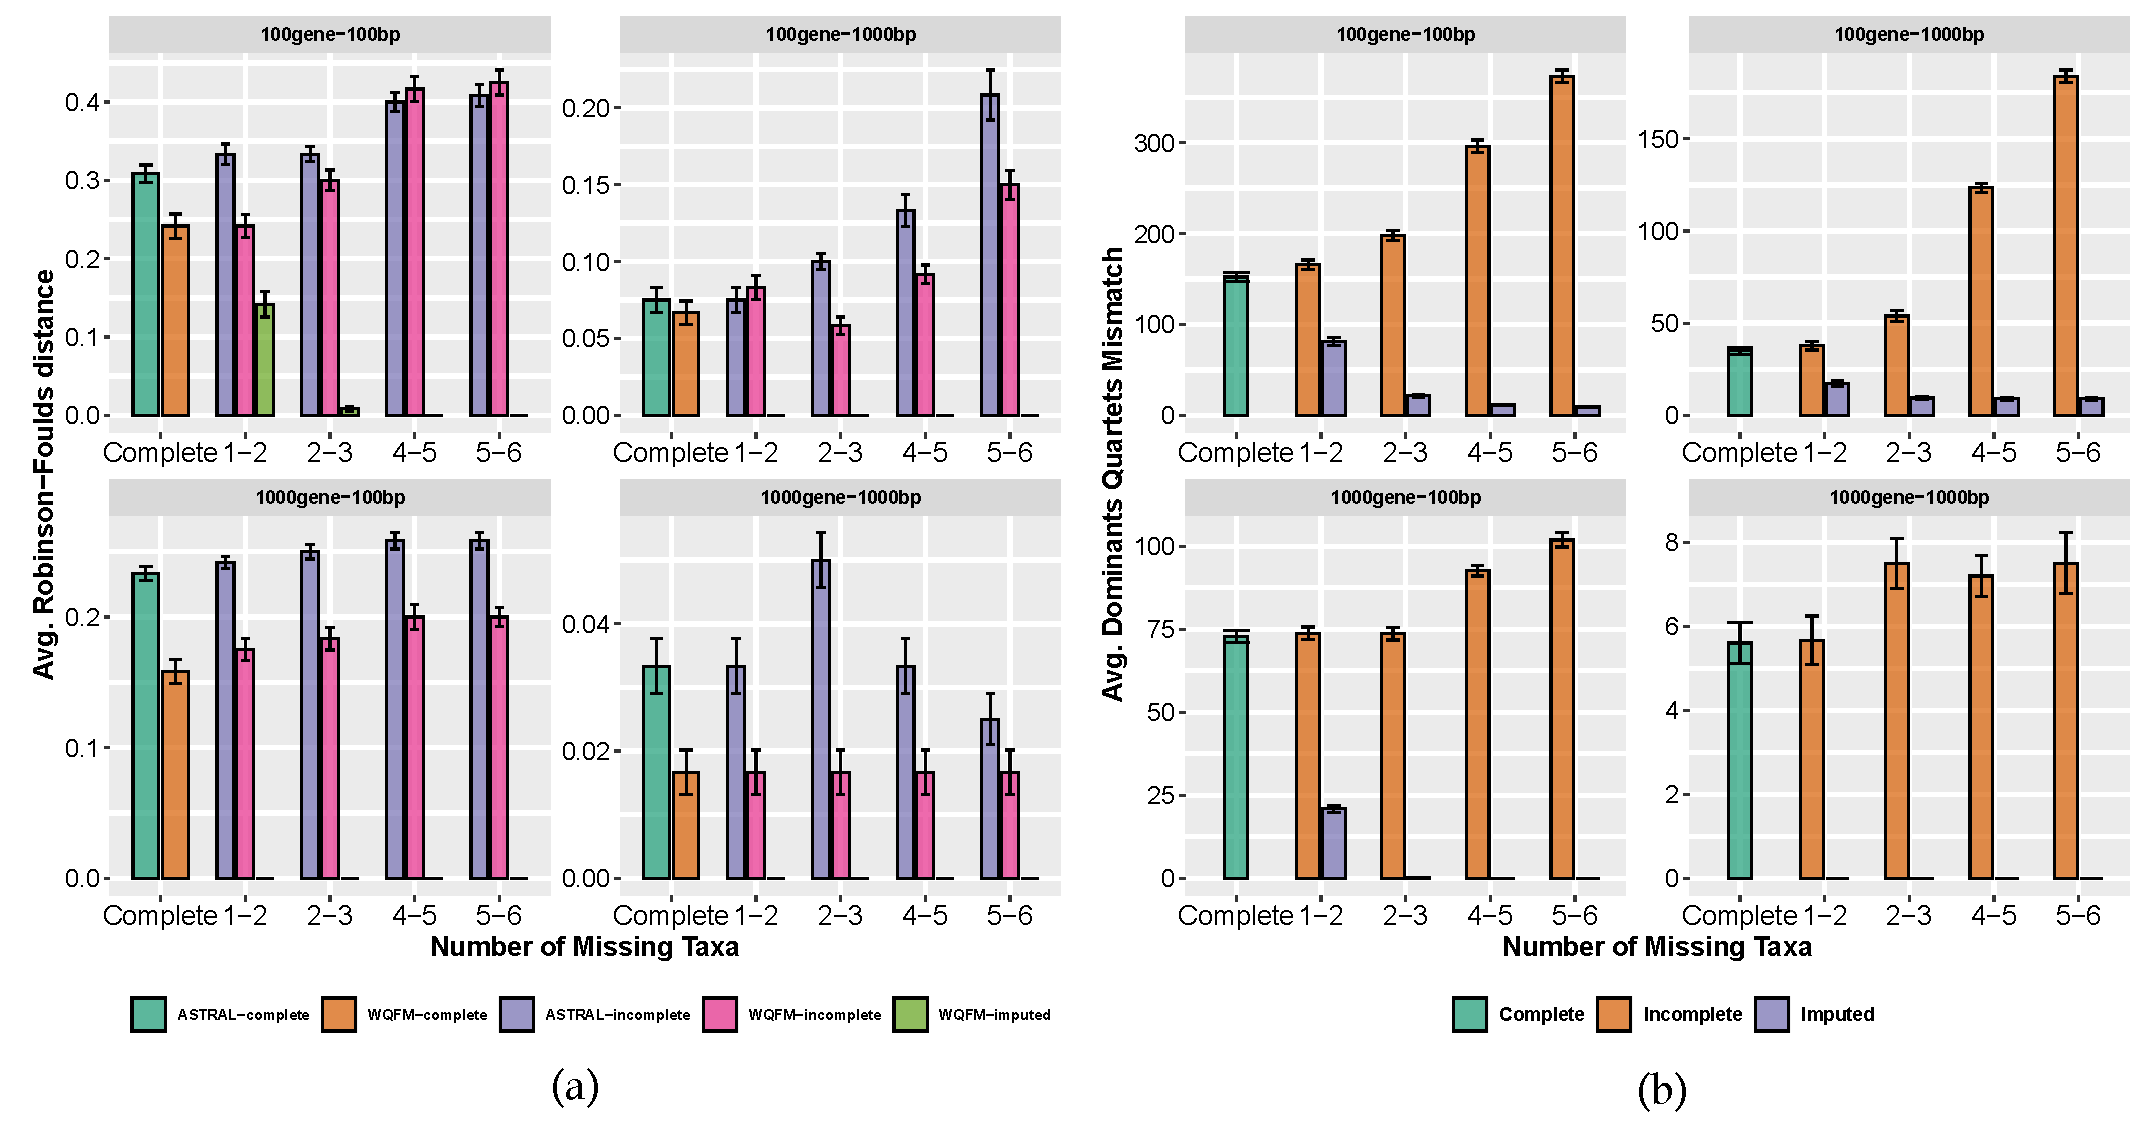
\includegraphics[width=\linewidth]{figures/15-taxon-combined.pdf}
    \caption{\textbf{Results on 15-taxon dataset.} (a) Comparison of different variants of ASTRAL and wQFM on 15-taxon dataset. We show the average RF rates with standard errors over 10 replicates. For each model condition, we varied the taxa removal rate from $\sim$6\% to $\sim$40\%, resulting in 13-80\% missing quartets. (b) Average numbers of dominant quartets (out of $15\choose4$) in different quartets distributions that differ from the true dominant quartets. }
    \label{fig:RF_Rates_15_taxon}
    \end{figure}


We performed a series of experiments to show the impact and quality of the quartet distributions produced by QT-GILD. First, we measure the divergence between true quartet distributions and different sets of quartet distributions in estimated gene trees (e.g., complete, incomplete and imputed) in terms of the number of ``dominant'' quartets that differ between two quartet distributions.
For a set of four taxa $a, b, c, d$, the dominant quartet (out of three possible quartets $ab|cd$, $ac|bd$, and $bc|ad$) is defined to be the quartet with the highest weight (i.e., the most frequent quartet topology). A dominant quartet topology is the statistically consistent estimate for the true evolutionary history among a group of four taxa since there are no \textit{anomalous} 4-leaf unrooted gene trees~\cite{degnan-rosenberg,degnan2013anomalous}. For a set of $n$ taxa, there are $n\choose4$ different four-taxa sets, and thus $n\choose4$ dominant quartets. In Fig.~\ref{fig:RF_Rates_15_taxon}(b), we show the numbers of dominant quartets (out of $15\choose4$) in complete, incomplete and imputed set of quartets that differ from the dominant quartets in true gene trees. Incomplete quartet distributions had the highest numbers of mismatches, followed by complete quartet distribution and the imputed sets of quartets incurred the lowest amount of mismatch (in most cases, the numbers of mismatches are $\sim$0), explaining why the RF rates of the trees estimated from imputed quartets are $\sim$0. The numbers of mismatches in incomplete quartet distributions increased as we increase the amount of missing data. In contrast, the numbers of mismatch in imputed quartet distributions decreased with increasing amounts of missing data (especially on model conditions with higher amounts of gene tree estimation error, ie., the 100-bp model condition). This is because, in the presence of higher numbers of missing quartets, QT-GILD had the opportunity to impute more quartets and in doing so it accounted for larger amounts of gene tree estimation error. This explains the seemingly counter-intuitive trend that RF rates of wQFM-imputed decreased with increasing amounts of missing data. %Figures~\ref{fig:RF_Rates_15_taxon} (a) and~\ref{fig:RF_Rates_15_taxon} (b) suggest that the lower numbers of mismatches result in lower RF rates -- a trend which is to be expected. 
Next, we measured the divergence between the quartet distribution of estimated gene trees and the quartet distribution of true gene trees using Jensen-Shannon divergence~\cite{jensen-shannon}. We represent the gene tree distribution by the frequency of each of the three possible alternative topologies for all the $n \choose 4$ quartets of taxa. Jensen-Shannon divergence of complete, incomplete and imputed quartet distributions from true quartet distributions are shown in Fig.~\ref{fig:JSD_15_taxon} in Appendix. The fact that the difference (both in terms of numbers of mismatch in dominant quartet topologies and Jensen-Shannon distance) between true and complete quartet distributions is higher than the difference between true and imputed quartet distributions suggests that QT-GILD not only imputes the missing quartets, but also accounts for gene tree estimation error. %by correcting the quartet distribution induced by estimated gene trees.
%Divergence of estimated gene trees triplet distributions from true gene tree distributions for simulated mammalian datasets
%we generate the distribution of 3$n \choose 4$ weighted quartets induced by a given set of gene trees. We measure the error in various quartet distributions, induced by complete and incomplete gene tree distributions using the deviation of quartet frequencies from the quartet frequency distribution computed using the true complete gene trees. For a set of $n$ taxa, we generate the distribution of 3$n \choose 4$ weighted quartets induced by a given set of gene trees. We used \add{Jansen-Shanon divergence or something else? add with reference} to measure the divergence between two sets of weighted quartets.  
Next, in order to show the efficacy of QT-GILD in imputing missing quartets, we report the proportion of missing quartets that were correctly imputed, with respect to both estimated and true gene trees, by QT-GILD (see Table \ref{tab:qstat-15} in Appendix). QT-GILD was able to correctly impute around 51-58\% and 51-63\% of missing quartets with respect to estimated and true gene trees, respectively. %Note that the proportion of correctly imputed quartets is higher when it was measured with respect to 


Finally, we computed the quartet scores of different species trees estimated by different methods with respect to both estimated and true gene trees (see Tables \ref{tab:qscore-15} and \ref{tab:qscore-15-true}.). Interestingly, on estimated gene trees, although ASTRAL obtained higher quartet scores than wQFM-incomplete, and wQFM-imputed in most of the model conditions, the scores of wQFM-incomplete and wQFM-imputed are closer to the true quartet score than the scores of ASTRAL-estimated trees are to the true score. This is mostly a result of the presence of gene tree estimation error. %and an evidence that wQFM works better than ASTRAL in general and that QT-GILD takes care of gene tree estimation error. 
The superiority of wQFM as a quartet-based tree estimation methods and the efficacy of QT-GILD as an imputation method are even more evident from the quartet scores when they are computed with respect to the true gene trees (i.e., no estimation error). 
Across all the model conditions, wQFM-imputed obtained the highest quartet scores (w.r.t true gene trees), followed by wQFM-complete and ASTRAL-complete (Table \ref{tab:qscore-15-true} in Appendix). The lowest scores were obtained when the gene trees are incomplete. Notably, wQFM-incomplete consistently achieved higher quartet scores than ASTRAL-incomplete. Note that the quartet consistency score is a statistical consistent measure meaning that the higher the quartet scores, the more accurate the species trees will be (given a sufficiently large number of true gene trees). Therefore, these quartet scores with respect to true gene trees support the trends observed in RF rates (see Fig.~\ref{fig:RF_Rates_15_taxon}). 

%These results clearly indicate that QT-GILD imputes as well as correct the quartet distribution, resulting in quartet distributions that are close to the true quartet distribution and thereby obtaining highly accurate species trees \addb{move this sentence to discussion}. 

%highly accurate species trees and well as demonstrate the impact of imputed quartets in inferring highly accurate species trees.



\begin{comment}
\begin{figure}[htbp]
    
    \includegraphics[width=\linewidth]{15_Taxon_Dataset/plot_QRF_Small.pdf}
    \caption{Comparison of different variants of ASTRAL and wQFM on 15-taxon dataset. We show the average RF rates with standard errors over 10 replicates. For each model condition, we varied the taxa removal rate from $\sim$6\% to $\sim$40\%.}
    \label{fig:RF_Rates_15_taxon}
    \end{figure}

\end{comment}

%\begin{table}[htbp]
  \small
  \centering
    \addtolength{\leftskip} {-2cm} % increase (absolute) value if needed
    \addtolength{\rightskip}{-2cm}
    \caption{Quartet statistics for 15-taxon dataset. For various model conditions with different numbers of missing taxa, we show the average number of quartets (present and missing) over 10 replicates. We also show what proportion of the missing quartets that were correctly imputed by QT-GILD with respect to both estimated and true gene trees.}
    \label{tab:qstat-15}
\begin{tabularx}{1.2\textwidth}{|X|X|X|X|X|X|X|}


\hline
Model & \# of Missing Taxa & \# of Quartets  &  \# of Missing Quartets &\% Missing Quartets & \% Correctly imputed (w.r.t estimated gene trees) &\% Correctly imputed (w.r.t. true gene trees) \\
    \hline \hline
    %do for all (difference)
    \multirow{4}{0.25\textwidth}{100gene-\\100bp} 
    & 0   & 136500 &    0.0  &    0.0   & --- & --- \\  \cline{2-7}
    & 1-2 & 118227.2  &	18272.8 & 13.39 & 54.67 & 52.20 \\ \cline{2-7}
    & 2-3 & 85288.8 &	51211.2 & 37.5 & 54.40 & 52.68 \\ \cline{2-7}
    & 4-5 & 41301.2 &	95198.8 & 69.74 & 51.73 & 52.23 \\ \cline{2-7}
    & 5-6 & 27046 &	109454 & 80 & 51.81 & 51.03 \\ \cline{2-7}
    \hline
    \multirow{4}{0.25\textwidth}{100gene-\\1000bp} 
    & 0   & 136500 &    0.0 &    0.0   &   --- &   --- \\  \cline{2-7}
    & 1-2 & 118119 &	18381 &    13.46 	&	55.72 &  63.18\\ \cline{2-7}
    & 2-3 & 85292 &     51207 &    37.5	&	54.96 &  62.72 \\ \cline{2-7}
    & 4-5 & 41291 &	    95209 &    69.7   &	54.30 &  60.03\\ \cline{2-7}
    & 5-6 & 27503 &	    108897 &    79.85  &	53.44  &   58.56\\ \cline{2-7}
    \hline
    
    \multirow{4}{0.25\textwidth}{1000gene-\\100bp} 
    & 0   & 1365000 &    0.0 &    0.0     & --- &   --- \\  \cline{2-7}
    & 1-2 & 1183509.6 &	181490.4 &    13.29  &	54.92 &   56.28 \\ \cline{2-7}
    & 2-3 & 858228.8 &	506771.2 &    37.12  &	54.42 &   56.34  \\ \cline{2-7}
    & 4-5 & 411790.5 &   953209.5 &    69.8  &	53.53 & 54.26 \\ \cline{2-7}
    & 5-6 & 269976 &	1095024 1 &    80.2  &	52.47 & 53.21 \\ \cline{2-7}
    \hline
    
    \multirow{4}{0.25\textwidth}{1000gene-\\1000bp} 
    & 0   & 1365000 &    0.0 &    0.0    & --- &  --- \\  \cline{2-7}
    & 1-2 & 1181069.8  & 183930.2 &    13.47 	& 58.04	 & 62.88  \\ \cline{2-7}
    & 2-3 & 857113.4 &	507886.6 &    37.2 	& 57.81	 &  62.76 \\ \cline{2-7}
    & 4-5 & 411361.5	&   953638.5 &    69.8 	& 56.44	 & 62.02  \\ \cline{2-7}
    & 5-6 & 270435 &	1094565 &    80.18 	& 55.38 &  	60.65  \\ \cline{2-7}
    \hline
    


\hline
    
\end{tabularx}

\end{table}

%% \setlength\LTleft{-1.0cm}% 2.5cm into the left margin
% \setlength\LTright{0pt plus 1fill minus 1fill}% whatever is needed at the right

\begin{table}[H]
  \small
  \centering
    \addtolength{\leftskip} {-2cm} % increase (absolute) value if needed
    \addtolength{\rightskip}{-2cm}
    \caption{Average quartet scores of the estimated and true species tree with respect to estimated gene trees for the 15-Taxon dataset. The quartet scores that are equal to the true species tree score are shown in bold and the highest quartet scores are shown in italic.}
    \label{tab:qscore-15}
\begin{tabularx}{1.2\textwidth}{|X|X|X|X|X|X|X|X|}


\hline
    Model & Number of Missing Taxa  & Complete (Astral)  & Complete (WQFM) & Incomplete (Astral) & Incomplete (WQFM)  &	Imputed (WQFM) & True Species Tree \\
    \hline\hline
    \multirow{4}{0.25\textwidth}{100gene-\\100bp} 
    & 0   & \textit{69933.8} & 69776.6 & --- & --- & --- & \multirow{4}{0.25\textwidth}{69307.4}  \\ \cline{2-7}
    & 1-2 & --- & --- &	\textit{69914.8} & 69784.1	
    & 69678.7 &  \\ \cline{2-7}
    & 2-3 & --- & ---  & \textit{69885.2} &	69632.9 
    &	69320.8 & \\ \cline{2-7}
    & 4-5 & ---	& ---  & \textit{69559.1} & 69366.6 	
    & \textbf{69307.4} & \\ \cline{2-7}
    & 5-6 & --- &	---	 &	69307.8	& 69179.2  
    & \textbf{\textit{69307.4}} & \\ \cline{2-7}
    \hline
    
    \multirow{4}{0.25\textwidth}{100gene-\\1000bp} 
    & 0 & \textit{82166.6} & 82109.2 & --- & --- & --- & \multirow{4}{0.25\textwidth}{82099.2}  \\ \cline{2-7}
    & 1-2 & --- & ---  &	\textit{82166.6} &	82146.4 
    &	\textbf{82099.2} &  \\ \cline{2-7}
    & 2-3 & --- &	---	 &	\textit{82106} &	82083 
    & \textbf{82099.2} &  \\ \cline{2-7}
    & 4-5 & --- &	---  & 81998.1	 &	82022.5  &	\textbf{\textit{82099.2}} &   \\ \cline{2-7}
    & 5-6 & --- &	---  &	81682.7 &	81761.3  &	\textbf{\textit{82099.2}} & \\ \cline{2-8}
    \hline
    
    \multirow{4}{0.25\textwidth}{1000gene-\\100bp} 
    & 0 & \textit{693656.1} & 692949.2 & --- & --- & --- & \multirow{4}{0.25\textwidth}{690268}  \\ \cline{2-7}
    & 1-2 & --- &	---  &	\textit{693648.1} &	693172.4  &	\textbf{690268} & \\ \cline{2-7}
    & 2-3 & --- &	---  &	\textit{693615.8} &	693008.6  &	\textbf{690268} &  \\ \cline{2-7}
    & 4-5 & --- &	---  &	\textit{693533.8} &	693117.7  &	\textbf{690268} &  \\ \cline{2-7}
    & 5-6 & --- &	---  &	\textit{693527.5} &	692743.1  &	\textbf{690268} & \\ \cline{2-7}
    \hline
        
    \multirow{4}{0.25\textwidth}{1000gene-\\1000bp} 
    & 0  & \textit{818022} &	817994 & --- & --- & --- &
    \multirow{4}{0.25\textwidth}{817937.3}  \\ \cline{2-7}
    & 1-2 & --- &	---- &	\textit{818021} &	8187994  &	\textbf{817937.3} &  \\ \cline{2-7}
    & 2-3 & --- &	--- &	\textit{818003.9} &	817993.9  &	\textbf{817937.3} &  \\ \cline{2-7}
    & 4-5 & --- & ---  &	\textit{818022.2} &	817993.9  &	\textbf{817937.3} &  \\ \cline{2-7}
    & 5-6 & --- &	--- &	\textit{817994} &	817993.9  &	\textbf{817937.3} & \\ \cline{2-7}
    \hline
    
\end{tabularx}

\end{table}


%% \setlength\LTleft{-1.0cm}% 2.5cm into the left margin
% \setlength\LTright{0pt plus 1fill minus 1fill}% whatever is needed at the right

\begin{table}[H]
  \small
  \centering
    \addtolength{\leftskip} {-2cm} % increase (absolute) value if needed
    \addtolength{\rightskip}{-2cm}
    \caption{Average quartet scores (over 10 replicates) of the estimated and true species trees with respect to true gene trees for the 15-Taxon dataset.  The quartet scores that are equal to the true species tree score are shown in bold and the highest quartet scores are shown in italic.}
    \label{tab:qscore-15-true}
\begin{tabularx}{1.2\textwidth}{|X|X|X|X|X|X|X|X|}


\hline
    Model & Number of Missing Taxa  & Complete (Astral)  & Complete (WQFM) & Incomplete (Astral) & Incomplete (WQFM)  &	Imputed (WQFM) & True species Tree \\
    \hline\hline
    \multirow{4}{0.25\textwidth}{100gene-\\100bp} 
    & 0   & 82158.6 & \textit{82708.3} & --- & --- & --- & \multirow{4}{0.25\textwidth}{ 84634.9}  \\ \cline{2-7}
    & 1-2 & --- & --- &	81790.7 & 82713.1	
    & \textit{83549.3} &  \\ \cline{2-7}
    & 2-3 & --- & ---  &	81947.2 &	82231.6 
    & \textit{84627.5} & \\ \cline{2-7}
    & 4-5 & ---	& ---  &	81213.6 & 80831.3	
    & \textbf{\textit{84634.9}} & \\ \cline{2-7}
    & 5-6 & --- &	---	 &	80699.4	& 80624  
    &	\textbf{\textit{84634.9}} & \\ \cline{2-7}
    \hline
    
    \multirow{4}{0.25\textwidth}{100gene-\\1000bp} 
    & 0 & 84345.1 & \textit{84366.1} & --- & --- & --- & \multirow{4}{0.25\textwidth}{84634.9}  \\ \cline{2-7}
    & 1-2 & --- & ---  &	82166.6 &	82146.4 
    &	\textbf{\textit{84634.9}} &  \\ \cline{2-7}
    & 2-3 & --- &	---	 &	82106 &	82083 
    & \textbf{\textit{84634.9}} &  \\ \cline{2-7}
    & 4-5 & --- &	---  & 81998.1	 &	82022.5  &	\textbf{\textit{84634.9}} &   \\ \cline{2-7}
    & 5-6 & --- &	---  &	81682.7 &	81761.3  &	\textbf{\textit{84634.9}} & \\ \cline{2-8}
    \hline
    
    \multirow{4}{0.25\textwidth}{1000gene-\\100bp} 
    & 0 & 827970.1	& \textit{834890.2} & --- & --- & --- & \multirow{4}{0.25\textwidth}{844184.3}  \\ \cline{2-7}
    & 1-2 & --- &	---  &	826981.3 &	833742.8  &	\textbf{\textit{844184.3}} & \\ \cline{2-7}
    & 2-3 & --- &	---  &	825679.5 &	832472.8  &	\textbf{\textit{844184.3}} &  \\ \cline{2-7}
    & 4-5 & --- &	---  &	824174.4 &	830065.4  &	\textbf{\textit{844184.3}} &  \\ \cline{2-7}
    & 5-6 & --- &	---  &	824202.9 &	831620.6  &	\textbf{\textit{844184.3}} & \\ \cline{2-7}
    \hline
        
    \multirow{4}{0.25\textwidth}{1000gene-\\1000bp} 
    & 0  & 843362.8 &	\textit{843791.8} & --- & --- & --- &
    \multirow{4}{0.25\textwidth}{844184.3}  \\ \cline{2-7}
    & 1-2 & --- &	---- &	818021 &	8187994  &	\textbf{\textit{844184.3}} &  \\ \cline{2-7}
    & 2-3 & --- &	--- &	842977 &	843791.8  &	\textbf{\textit{844184.3}} &  \\ \cline{2-7}
    & 4-5 & --- & ---  &	843362.8 &	843791.8  &	\textbf{\textit{844184.3}} &  \\ \cline{2-7}
    & 5-6 & --- &	--- &	843162.5 &	843791.8  &	\textbf{\textit{844184.3}} & \\ \cline{2-7}
    \hline
    
\end{tabularx}

\end{table}


